\documentclass[9pt,twocolumn,twoside]{pnas-new}\usepackage[]{graphicx}\usepackage[dvipsnames]{xcolor}
% maxwidth is the original width if it is less than linewidth
% otherwise use linewidth (to make sure the graphics do not exceed the margin)
\makeatletter
\def\maxwidth{ %
  \ifdim\Gin@nat@width>\linewidth
    \linewidth
  \else
    \Gin@nat@width
  \fi
}
\makeatother

\definecolor{fgcolor}{rgb}{0.345, 0.345, 0.345}
\newcommand{\hlnum}[1]{\textcolor[rgb]{0.686,0.059,0.569}{#1}}%
\newcommand{\hlstr}[1]{\textcolor[rgb]{0.192,0.494,0.8}{#1}}%
\newcommand{\hlcom}[1]{\textcolor[rgb]{0.678,0.584,0.686}{\textit{#1}}}%
\newcommand{\hlopt}[1]{\textcolor[rgb]{0,0,0}{#1}}%
\newcommand{\hlstd}[1]{\textcolor[rgb]{0.345,0.345,0.345}{#1}}%
\newcommand{\hlkwa}[1]{\textcolor[rgb]{0.161,0.373,0.58}{\textbf{#1}}}%
\newcommand{\hlkwb}[1]{\textcolor[rgb]{0.69,0.353,0.396}{#1}}%
\newcommand{\hlkwc}[1]{\textcolor[rgb]{0.333,0.667,0.333}{#1}}%
\newcommand{\hlkwd}[1]{\textcolor[rgb]{0.737,0.353,0.396}{\textbf{#1}}}%
\let\hlipl\hlkwb

\usepackage{framed}
\makeatletter
\newenvironment{kframe}{%
 \def\at@end@of@kframe{}%
 \ifinner\ifhmode%
  \def\at@end@of@kframe{\end{minipage}}%
  \begin{minipage}{\columnwidth}%
 \fi\fi%
 \def\FrameCommand##1{\hskip\@totalleftmargin \hskip-\fboxsep
 \colorbox{shadecolor}{##1}\hskip-\fboxsep
     % There is no \\@totalrightmargin, so:
     \hskip-\linewidth \hskip-\@totalleftmargin \hskip\columnwidth}%
 \MakeFramed {\advance\hsize-\width
   \@totalleftmargin\z@ \linewidth\hsize
   \@setminipage}}%
 {\par\unskip\endMakeFramed%
 \at@end@of@kframe}
\makeatother

\definecolor{shadecolor}{rgb}{.97, .97, .97}
\definecolor{messagecolor}{rgb}{0, 0, 0}
\definecolor{warningcolor}{rgb}{1, 0, 1}
\definecolor{errorcolor}{rgb}{1, 0, 0}
\newenvironment{knitrout}{}{} % an empty environment to be redefined in TeX

\usepackage{alltt}
% Use the lineno option to display guide line numbers if required.
\usepackage{cleveref}
\usepackage[dvipsnames]{xcolor} % colors
\newcommand{\svp}[1]{{\textcolor{RedOrange}{#1}}}
\newcommand{\hh}[1]{{\textcolor{ForestGreen}{#1}}}
\newcommand{\ac}[1]{{\textcolor{Purple}{#1}}}
\templatetype{pnasbriefreport}
%\templatetype{pnasbriefreport} % Choose template
% {pnasresearcharticle} = Template for a two-column research article
% {pnasmathematics} %= Template for a one-column mathematics article
% {pnasinvited} %= Template for a PNAS invited submission

\title{Hidden Multiple Comparisons Increase Forensic Error Rates}

% Use letters for affiliations, numbers to show equal authorship (if applicable) and to indicate the corresponding author
\author[a,1,2]{Susan Vanderplas}
\author[b, c]{Alicia Carriquiry}
\author[b, c, 1]{Heike Hofmann}

\affil[a]{Statistics Department, University of Nebraska Lincoln. 350 Hardin Hall, 3310 Holdrege North Wing, Lincoln, NE 68503}
\affil[b]{Department of Statistics, Iowa State University. 1121 Snedecor Hall, 2438 Osborn Dr, Ames, IA 50011}
\affil[c]{Center for Statistics and Applications in Forensic Evidence. 195 Durham Center, 613 Morrill Road, Ames, Iowa 50011}

% Please give the surname of the lead author for the running footer
\leadauthor{Vanderplas}

% Please include corresponding author, author contribution and author declaration information
\authorcontributions{Please provide details of author contributions here.}
\authordeclaration{The authors have no competing interests to declare.}
\equalauthors{\textsuperscript{1}SVP (Author One) contributed equally to this work with HH (Author Two).}
\correspondingauthor{\textsuperscript{2}To whom correspondence should be addressed. E-mail: susan.vanderplas@unl.edu}

% At least three keywords are required at submission. Please provide three to five keywords, separated by the pipe symbol
\keywords{Forensic Evidence $|$ Statistics $|$ Wire cuts $|$ Toolmark analysis}


\begin{abstract}
When wires are cut, the tool produces striations on the cut surface; as in other forms of forensic analysis, these striation marks are used to connect the evidence to the source that created them. Here, we argue that the practice of comparing two wire cut surfaces introduces complexities not present in better-investigated forensic examination  of toolmarks such as those observed on bullets, as wire comparisons inherently require multiple distinct comparisons, increasing the expected false positive rate. We call attention to the multiple comparison problem in wire examination and relate it to other situations in forensics that involve multiple comparisons, such as database searches.
\end{abstract}

\dates{This manuscript was compiled on \today}
\doi{\url{www.pnas.org/cgi/doi/10.1073/pnas.XXXXXXXXXX}}


\IfFileExists{upquote.sty}{\usepackage{upquote}}{}
\begin{document}

\maketitle
\thispagestyle{firststyle}
\ifthenelse{\boolean{shortarticle}}{\ifthenelse{\boolean{singlecolumn}}{\abscontentformatted}{\abscontent}}{}





\firstpage[7]{5}

\dropcap{I}n forensic evaluations, a single conclusion often relies on  many comparisons, either implicitly or explicitly.
Multiple comparisons arise persistently when developing statistical methods to address scientific problems \citep{benjaminiControllingFalseDiscovery1995}, and greatly increase the probability of false discoveries.
Now that vast databases and efficient algorithms are routinely used in forensic evaluations to propose matches to crime scene items, the problem of close non-matches~\citep{pcast} due to multiple comparisons becomes critically important.
This often ignored issue increases the false positive rate, and can contribute to the erosion of public trust in the justice system.
The multiple comparison problem is not new: it has been raised in the past with regard to DNA~\citep{thompson2003} and latent print evaluations~ \citep{koehler2021}. One of the root causes~\citep{fine2006} leading to the wrongful accusation of Brandon Mayfield in the 2004 Madrid train bombing case was that the large size of the IAFIS database used to search for similar prints made it possible to locate `unusually' close non-matches.
% The probability of finding  close non-matches for an item of evidence is proportional to the size of the database available for searching; close non-matches occur more frequently as databases increase in size.
\svp{As database size increases, so does the probability of finding a close non-match.}

Compounding this issue, the use of algorithms also results in a large number of comparisons that are not obvious to the user.
For example, the cross-correlation function~\citep{vorburgerApplicationsCrosscorrelationFunctions2011} was one of the first measures proposed for quantifying the similarity between two patterns in response to the 2009 NRC report~\citep{nas2009}, and continues to be used in many pattern searching algorithms to find the best alignment between two images and to quantify their overall similarity.
Finding the best alignment often consists in sliding one surface across the whole length (for one-dimensional patterns, such as striations) or area (for two dimensional sources, such as impression marks) of the other item while keeping track of the value of a similarity measure.
This mirrors the forensic examination process: the examiner visually rotates and shifts items under a comparison microscope to align two surfaces.
In order to avoid false accusations and further erosions of public trust in science, we must address the problem of multiple comparisons and control their effect on false discovery rates.

Here, we consider the multiple comparisons problem that arises from a relatively simple toolmark examination: matching a cut wire to a wire-cutting tool.
We describe the comparison approach, estimate the (minimal) number of comparisons that are needed to carry out the examination, and discuss how the false discovery rate changes with the number of comparisons involved, using error rates derived from published black-box studies.


\section*{Examination Process}

A forensics examiner tasked with determining whether a wire in evidence was cut by a specific tool will create one or more blade cuts using the putative tool, which are then compared to the cut surface of the wire.
These cuts are made in a sheet of material similar to the wire's composition, and may be performed at multiple angles, as the angle of the tool to the substrate can affect which striations are recorded on the substrate surface.
The blade cuts will then be compared to the wire under a comparison microscope, though eventually, automatic comparison algorithms may also be validated for lab use.
Each side of each blade cut will be compared to each side of the wire;
\svp{different tool designs have between 2 and 4 cutting surfaces in contact with the substrate.}
% depending on the tool design, there can be between two and four cutting surfaces in contact with the substrate.

\section*{Calculating the Number of Comparisons}

In order to calculate the number of comparisons carried out in the course of one examination, we define $\ell$ to be the length of the blade cut, and $d$ to be the diameter of the wire.
We assume that the wire is covered with striations suitable for comparison across its full diameter $d$.
If this is not the case, we reduce the value $d$.
Both the blade and the wire are either digitally scanned at resolution $r$ mm per pixel, or visually examined using a microscope with a digital resolution that can be expressed as $r$ equivalent to the digital scan.
An illustration of the sliding comparison process is shown in \Cref{fig:wire-blade}.
Imagine that we move the cut wire along the blade cut in order to assess whether striations on the blade cut match the striations on the wire.
We can move the wire unit-by-unit, or we can move the wire by its full length, with no overlap to the previous comparison.

The first option gives us the maximum number of comparisons ($\ell/r - d/r + 1$), while the second option gives us the minimum number of comparisons $\ell/d$.
In the first case, sequential comparisons share much of the same physical data and are highly related; in the second case, no data are shared between physical comparisons and we can expect that they are statistically independent, though empirically there will be nonzero correlations due to physical similarities between striations.
For simplicity, let us consider the number of comparisons to lie somewhere between these two estimates.
Note that when $\ell/d \approx 1$, as in some toolmark comparisons, the upper number of comparisons goes to 1.
Finally, we must consider the number of surfaces which must be compared: the wire may have one or two sets of striae and there may be  two to four blade cut surfaces to examine, depending on the tool.
This results in a multiplier of as much as 8.

\subsection*{A concrete example}



\begin{figure}[t!]
\centering
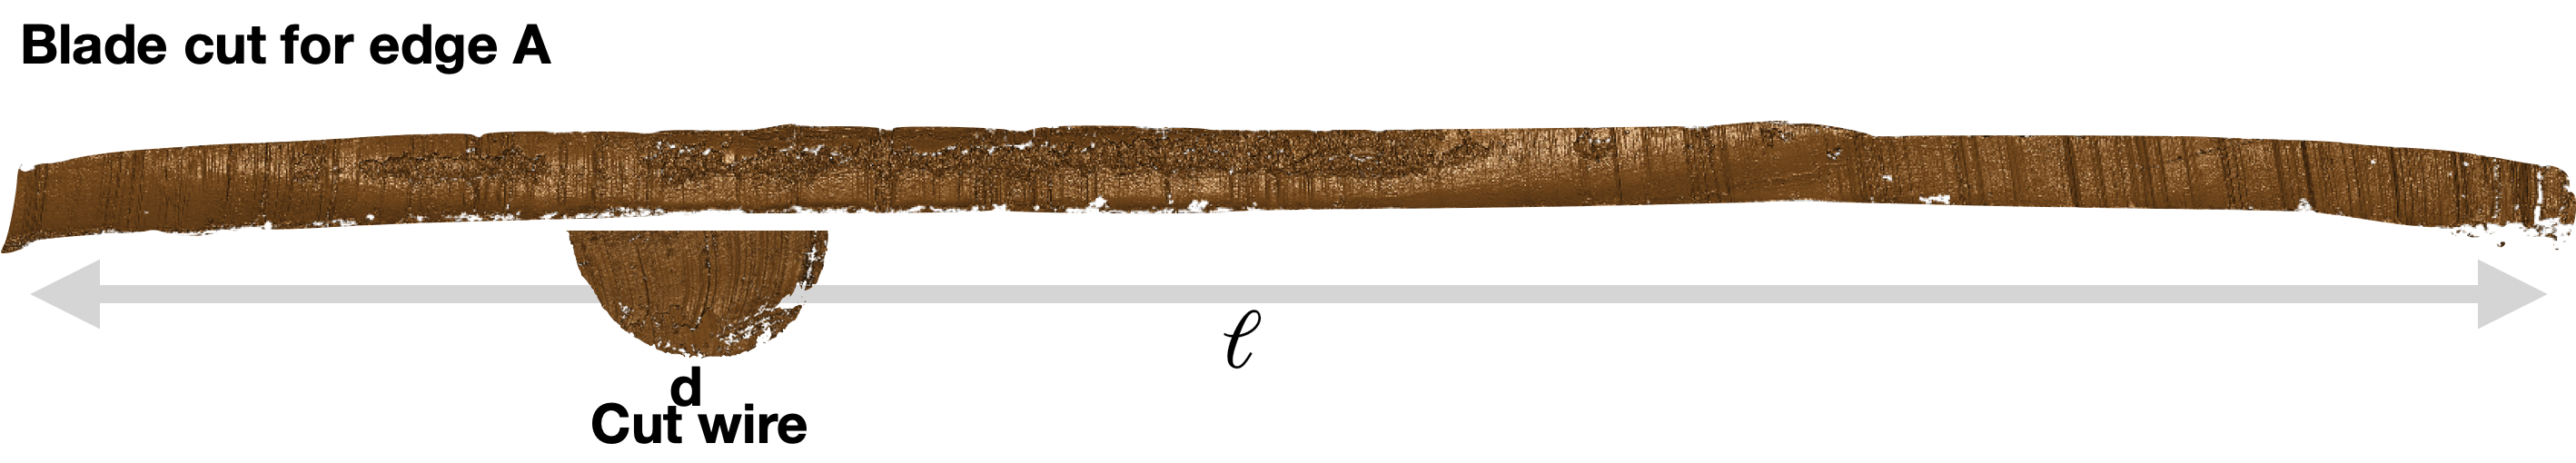
\includegraphics[width=\columnwidth]{../fig/wire-blade-comparison-label.png}
\includegraphics[width=\columnwidth]{../fig/wire_cutter_wires.png}
\caption{(Top) A comparison between a wire and a blade cut requires sliding the wire along the entire blade cut length to determine the best match (or whether there is a match). Surfaces shown are rendered 2D topographical scans of a wire and blade cut taken with a confocal light microscope. (Bottom) RJ45 Crimp tool with a $1.5$ cm razor blade used for cutting. 1 mm and 2 mm diameter aluminum wires cut with the pliers are shown in a box in the top right corner.}\label{fig:tool-pic}\label{fig:wire-blade}
\end{figure}

Let us consider a wire-cutting tool with a $1.5$ cm razor blade that meets a cast surface (one such tool is shown in \Cref{fig:tool-pic}); the wire is held against this rectangular cast surface as the blade is pushed into the wire, splitting it in two.
This is a minimal scenario - the wire will acquire striations from one side of the blade, while the blade itself has two cutting edges, which we will call side A and side B.
A blade cut of a sheet of aluminum will thus produce two striated edges corresponding to side A and side B which are compared to cut wires to assess similarity.
We also have a 12 gauge aluminum wire ($2$ mm diameter) which may have been cut by the wire-cutting tool described above.
Class characteristics, which are shared by all tools of similar manufacture, appear to match:
there is a flat impression on one side of the wire corresponding to the cast metal backstop of the tool,
and the wire is cut such that the blade and the backstop appear to be perpendicular
(that is, the wire appears to have been cut with a tool of similar configuration).
In this example, $\ell = 15$ mm, $d = 2$ mm, and there are at least $\ell/d = 7.5$ comparisons between a wire cut and a blade cut.
As there are two blade cuts (side A and side B), the minimal number of comparisons overall is 15, as these comparisons are non-overlapping and independent (on average).

Assuming a resolution of $0.645 \mu$m per pixel, the maximum number of comparisons per blade cut is around $20,000$; thus, we need $40,000$ comparisons overall in order to find the optimal alignment between the wire and the blade cut.
These comparisons are implicit in the calculation of cross-correlation, which is the first and often the only step used to quantitatively assess the similarity between striated evidence such as bullets, aperture shear, and firing pin impressions.
Implicit comparisons are not unique to algorithms; an examiner would need to physically align the wire and the blade cut by searching along the length of the cut to visually match striations, performing the same process physically that the algorithm performs computationally.
While these sequential comparisons are highly auto correlated, and we cannot assume sequential independence when calculating the probability of an error, they serve as an upper bound on the number of comparisons which could be performed.
As the number of comparisons increases, the probability of encountering a coincidental match increases.
Statisticians call this the \textit{family-wise error rate} $E$; it is an important quantity to control when conducting a series ("family") of tests.


\section*{Probability of False Identifications}
There are at least two components of the false positive rate (FPR): identifying two pieces of evidence that have similar characteristics but are from different sources (a coincidental match) and procedural failures (e.g.\ lab process errors) \citep[p 50]{pcast}.
In objective disciplines with standardized evaluation rules (e.g.\ DNA), these sources can be distinguished.
However, in toolmark examination, no objective evaluation rules are used; examiners testify based on subjective, individual rules for how much similarity is sufficient for an identification.
Assuming that lab procedure errors are not a factor in studies, we use reported error rates from open-set studies of striated evidence comparisons to estimate the coincidental match rate of a single wire-cut comparison.
The three studies we consider \citep{bajic2020, mattijssen2021,best2022} have FPRs between 0.0045 \citep{best2022} and 0.072 \citep{mattijssen2021}; pooling data from these studies yields an FPR of 0.02.
For a single-comparison FPR of $e$, the family-wise FPR for $n$ comparisons, $E_n$ is $1 - [1-e]^n$.
\Cref{tab:family-wise} \hh{shows the impact the number of comparisons has on these published error rates. With an error rate of 0.07, as suggested by Bajic (2020), examiners can make up to 14 comparisons, i.e.} \svp{even the simple example in this paper exceeds} \hh{an upper bound of 10\% for the family wise false identification error.}
%\Cref{tab:Accuracy} shows the family-wise accuracy rate on the y-axis; if 90\% is an acceptable overall accuracy, 2 comparisons can be made when $e = 0.05$; increasing to 10 comparisons when $e =  0.01$.
%Thus, at an error rate of sprintf("e = %.2f", fpr), examiners can conduct comparisons before exceeding the family-wise FPR of 10\%.
\svp{To conduct a search of a modestly sized database with 1000 entries, the initial FPR cannot}
% \hh{For a modestly sized database search of size 1000, the initial false positive rate should not
\hh{exceed 1 in 10,000 to guarantee a family-wise total false identification error of at most 10\%. }

Under these constraints, the accuracy of an examination involving multiple comparisons between a wire and a tool will be low, as the number of candidate alignments that must be examined is high.
Even the most innocuous example (small blade, only 2 cutting surfaces, and a relatively large wire) involves a minimum of 15 %completely independent
comparisons.
Examiners would make cuts under multiple angles \citep{baikerToolmarkVariabilityQuality2015}, increasing the number of comparisons \svp{and making a} false identification even more \svp{probable}.
As a result, it is questionable whether wire comparisons made under current protocols are reliable enough to be presented at trial.

\svp{Clearly, studies for wire evidence, and larger studies for striated evidence in general, are necessary.}
% \hh{Obviously, we need studies for wire evidence. It is also clear, based on the error rates, that larger studies are needed. }
\svp{Moving away from binary assessments toward quantification of striation similarity and observed pattern frequency will also reduce the severity of this issue and allow examiners to assign unusual striation patterns more weight in the process.}
% \hh{Going forward, we need to move away from  the binary assessment of 'match' or 'non-match' and quantify (a) the similarity of striations expressed between two pieces of evidence, and (b) the frequency of the observed pattern. Unusual striation patterns should be assigned more weight in the process.  }






\begin{table}
\scalebox{.95}{
\begin{tabular}{lcrrrr}
\toprule
 &  & \multicolumn{3}{p{25mm}}{False Positives (\%) in N comparisons} &  \\
\cmidrule(lr){3-5}
Study & FPR $e$ & $E_{10}$ & $E_{100}$ & $E_{1,000}$ & $E_N < 0.1$ \\
\midrule\addlinespace[2.5pt]
Mattijssen (2021) & 7.24\% & $52.8$ & $99.9$ & $100.0$ & $1$ \\
Pooled Error & 2.00\% & $18.3$ & $86.7$ & $100.0$ & $5$ \\
Bajic (2020) & 0.70\% & $6.8$ & $50.7$ & $99.9$ & $14$ \\
Best (2022) & 0.45\% & $4.5$ & $36.6$ & $98.9$ & $23$ \\
 & 1 in 1,000 & $1.0$ & $9.5$ & $63.2$ & $105$ \\
 & 1 in 10,000 & $0.1$ & $1.0$ & $9.5$ & $1,053$ \\
 & 1 in 100,000 & $10^{-4}$ & $0.1$ & $1.0$ & $10,535$ \\
\bottomrule
\end{tabular}}
\caption{\label{tab:family-wise}Table showing the relationship between false positive rates and the chance of false identifications in $N$ comparisons for a set of different FPRs and different number of comparisons. The last column gives the number of comparisons allowed while ensuring a false identification percentage of at most 10\%.}
\end{table}

\section*{Discussion \& Conclusions}

Forensic practitioners often report the findings from their examinations in the form of a categorical conclusion reflecting a single decision.
This is misleading when the decision relies on multiple comparisons which are not individually presented in reports or testimony.
In this short contribution, we have shown that the implicit comparisons performed during forensic analysis of wire cuts increase the family-wise error rate.
%Omission of the underlying details is not necessarily due to malice; rather, it results from protocols which focus on finding the best possible match between two items and evaluating that match.

We describe a simple scenario where a wire is cut using a two-sided blade, but findings apply to any situation where a forensic evaluation involves multiple comparisons, including, e.g., database searches.  Forensic practitioners should understand how the number of comparisons can affect the accuracy of their final conclusion. We propose three strategies to enhance transparency and enable more reliable estimates of examination-specific error rates.
%In our example we highlight a simple case where a wire is cut using a two-sided blade, but the findings apply to many other situations where a forensic evaluation involves multiple comparisons against a set of accumulated information, such as database searches.
%It is critically important that forensic practitioners become aware of the impact of carrying out multiple comparisons on their final conclusions and that lab procedures and testimony are modified accordingly.
%We suggest three strategies to improve transparency of forensic examinations and to produce more reliable estimates of examination-wide error rates.

First, examiners should report (or defense attorneys should request) the overall length or area of surfaces generated during the examination process, along with the total consecutive length or area of the recovered evidence.
These pieces of information will take the place of $\ell$ and $d$ and facilitate calculation of examination-wide error rates.

Second, researchers should conduct studies relating the length/area of comparison surface to the error rate.
For instance, we have pooled studies looking at bullet striations and firing pin shear marks because we could not find black-box error rate studies of wire cuts.
The striated surfaces are of orders of magnitude different lengths, but represent the best estimate of the error rate for striated materials.
New studies should be Type II studies as defined by Koehler \citep{koehlerIntuitiveErrorRate2017a}, designed to assess the actual error rate when examiners are making difficult comparisons.

Finally, when databases are used at any stage of the forensic evidence evaluation process (from suitability assessment and triage to reports which will be used at trial), the number of database items searched (or comparisons made) and the number of results returned must be reported.
Additionally, the number of results used for further manual comparison should also be reported.
For example, if a firearms examiner searches a local NIBIN database with 1000 entries, requests the 20 closest matches to her evidence, and then carries out a physical examination of five exemplars from the list of 20, all of those values should be clearly reported to enable estimation of the examination-wise error rate.
This will help make the multiple comparison issue accessible to everyone involved in evaluating the value of forensic evidence, from examiners to lawyers to jurors and judges.


\acknow{This work was funded (or partially funded) by the Center for Statistics and Applications in Forensic Evidence (CSAFE) through Cooperative Agreements 70NANB15H176 and 70NANB20H019 between NIST and Iowa State University, which includes activities carried out at Carnegie Mellon University, Duke University, University of California Irvine, University of Virginia, West Virginia University, University of Pennsylvania, Swarthmore College and University of Nebraska, Lincoln.}

\showacknow{} % Display the acknowledgments section

\bibliography{../references}
\end{document}
